% !TeX spellcheck = russian-aot
%\documentclass[12pt,a4paper,draft]{article}
%\usepackage{cmap}
%\usepackage[utf8]{inputenc}
%\usepackage[T2A]{fontenc}
%\usepackage[english,german,russian]{babel}
%\usepackage{amsmath}
%\usepackage{amsfonts}
%\usepackage{amssymb}
%\usepackage[final]{graphicx}
%\DeclareGraphicsExtensions{.jpg,.png}
%\graphicspath{{pictures/}} % путь к графическим файлам. Пусть они помещаются в подкаталог pictures текущего каталога
%\usepackage[figurename=Рисунок,labelsep=period]{caption}
%\usepackage{float}
%\usepackage{indentfirst}
%\usepackage[pdftex,left=2.5cm,right=2.5cm,top=3cm,bottom=3cm]{geometry}
%\usepackage[obeyDraft]{todonotes}
%\usepackage[hidelinks,draft=false]{hyperref}
%\frenchspacing
%\pdfcompresslevel=9

\documentclass[a4paper,12pt]{article}
\usepackage[utf8]{inputenc}
\usepackage[T2A]{fontenc}
\usepackage[english,russian]{babel}
\usepackage{natbib}
\usepackage[final]{graphicx}
\DeclareGraphicsExtensions{.jpg,.png}
\graphicspath{{pictures/}}
\usepackage{float}
\usepackage{amsmath}
\usepackage{pgfplots}
\usepackage{color} %% это для отображения цвета в коде
%\usepackage{listings} %% собственно, это и есть пакет listings




%\setmonofont{Consolas} %to be used with XeLaTeX or LuaLaTeX
\definecolor{bluekeywords}{rgb}{0,0,1}
\definecolor{greencomments}{rgb}{0,0.5,0}
\definecolor{redstrings}{rgb}{0.64,0.08,0.08}
\definecolor{xmlcomments}{rgb}{0.5,0.5,0.5}
\definecolor{types}{rgb}{0.17,0.57,0.68}

\usepackage{listings}
\lstset{
language=[Sharp]C,
captionpos=t,
%numbers=left, %Nummerierung
%numberstyle=\tiny, % kleine Zeilennummern
frame=lines, % Oberhalb und unterhalb des Listings ist eine Linie
showspaces=false,
showtabs=false,
breaklines=true,
showstringspaces=false,
breakatwhitespace=true,
escapeinside={(*@}{@*)},
commentstyle=\color{greencomments},
morekeywords={partial, var, value, get, set},
keywordstyle=\color{bluekeywords}\bf,
stringstyle=\color{redstrings},
basicstyle=\ttfamily\small,
extendedchars=\true
}

\usepackage{caption}
\DeclareCaptionFont{white}{\color{white}} %% это сделает текст заголовка белым
%% код ниже нарисует серую рамочку вокруг заголовка кода.
\DeclareCaptionFormat{listing}{\colorbox{gray}{\parbox{\textwidth}{#1#2#3}}}
\captionsetup[lstlisting]{format=listing,labelfont=white,textfont=white}


\usepackage{ctable}%для таблиц
\captionsetup[table]{justification=raggedleft,singlelinecheck=off}

%%%%%%%%%%%%%%%%%%%%%%%%%%%%%%%%%%%%%%%%%%%%%%%%%%%%%%%%%%%%%%%%%%%%%%%%%%%%%%%%%%%%%%%%%%%%%%%

\begin{document}
\begin{titlepage}
	\centering
    \begin{figure}[H]
    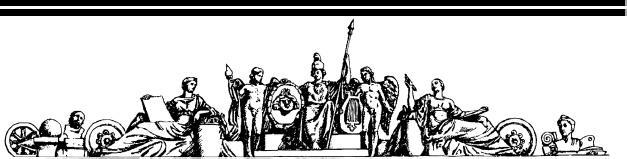
\includegraphics[width = 120mm]{photo}
    \end{figure}
	{\scshape Министерство образования Российской Федерации
Московский Государственный Технический Университет им. Н.Э. Баумана \par}
	\vspace{4cm}
	{\scshape\Large Отчёт по лабораторной работе № 1\par}
    {\scshape\Large По курсу: "Анализ алгоритмов"\par}
	{\scshape\Large\bf Тема:"Алгоритм Левенштейна"\par}
    \vspace{4cm}
    {\flushright Студент: Орехова Екатерина ИУ7-51\par}
    \vspace{4cm}
% Bottom of the page
	{\large \today\par}
\end{titlepage}

\def\contentaname{Содержание}
\tableofcontents %Вывод содержания
\clearpage

\section{Постановка задачи}
    В ходе выполнения лабораторной работы необходимо изучить алгоритм Левенштейна. Реализовать базовый алгоритм Левенштейна, рекурсивный алгоритм Левенштейна, модифицированный алгоритм Левенштейна. Сравнить эти алгоритмы.

\section{Описание алгоритма}
    Расстояние Левенштейна (также редакционное расстояние или дистанция редактирования) между двумя строками в теории информации и компьютерной лингвистике это минимальное количество операций вставки одного символа, удаления одного символа и замены одного символа на другой, необходимых для превращения одной строки в другую.
    Допустимы редакторские операции:
    \begin{itemize}
      \item D (delete) — удалить,
      \item I (insert) — вставить,
      \item R (replace) — заменить,
      \item M (match) — совпадение.
    \end{itemize}
    Модификацией данного алгоритма является алгоритм Дамерау — Левенштейна, суть которого заключается в добавлении ещё одной редакторской операции : C(change) – перестановки двух соседних символов.
    Пусть w(x) – цена операции х, тогда:
    \begin{itemize}
      \item w(D) = 1
      \item w(I) = 1
      \item w(R) = 1
      \item w(M) = 0
      \item w(C) = 1
    \end{itemize}

    \subsection{Рекурсивный алгоритм}
        Пусть $S_1$ и $S_2$ – две строки (длиной M и N) соответственно, тогда редакционное расстояние можно подсчитать по следующей рекуррентной формуле $d(S_1,S_2)=D(M,N)$ где
        \begin{equation*}
            D[i][j] =
            \begin{cases}
                0, \qquad \text{если $i=0, j=0$;}\\
                i, \qquad \text{если $j=0,i>0$;}\\
                j, \qquad \text{если $i=0,j>0$;}\\
                min\{D(i,j-1)+1,D(i-1,j)+1,D(i-1,j-1)+m(S_1 [i],S_2 [j])\},\\ \text{если $i>0,j>0$.}
            \end{cases}
        \end{equation*}
        где m(a,b) равна нулю, если a=b и единице в противном случае;\\
        $\min(a,b,c)$ возвращает наименьший из аргументов.

    \subsection{Матричный алгоритм}
    Матричный алгоритм можно описать с помощью следующей иллюстрации
    \begin{figure}[H]
    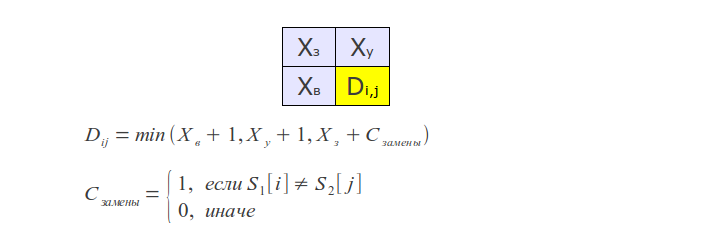
\includegraphics[scale=0.7]{leven}
    \caption{Матричный алгоритм}
    \end{figure}
    \subsection{Модифицированный алгоритм}
    Модифицированный алгоритм добавляет ещё одну операцию: перестановка двух соседних символов (или как по другому её называют - транспозиция)
    Модификацию матричного алгоритма можно представить следующей иллюстрацией
    \begin{figure}[H]
    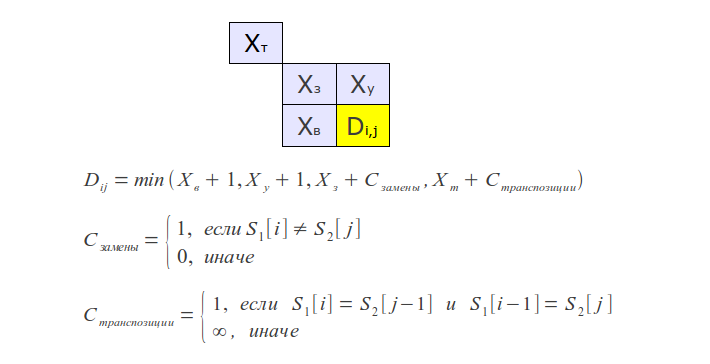
\includegraphics[scale=0.7]{levenmod}
    \caption{Модифицированный алгоритм}
    \end{figure}
\section{Реализация}
\begin{lstlisting}[label=some-code,caption={main}]
static void Main(string[] args)
{
    string word1 = Console.ReadLine();
    string word2 = Console.ReadLine();
    int len1, len2;
    len1 = word1.Length;
    len2 = word2.Length;
    // ооооо \ у\ 2\ 3

    functions.max = Math.Max(len1, len2) + 1;
    int d = functions.distance_rec(word1, word2, len1 - 1, len2 - 1);
    int d1 = functions.distance_matr(word1, word2, len1, len2);
    int dmod = functions.distance_modify(word1, word2, len1, len2);

    Console.Write("Levenshtein distance recursion " + d.ToString() + "\n");
    Console.Write("Levenshtein distance matrix " + d1.ToString() + "\n");
    Console.Write("Levenshtein distance matrix modify " + dmod.ToString() + "\n");
    Console.Read();
}
\end{lstlisting}

\begin{lstlisting}[label=some-code1,caption={Рекурсивный алгоритм}]
public static int distance_rec(string word1, string word2, int len1, int len2)
{
    if (len1 == -1)
    {
        if (len2 == -1)
            return 0;
        return len2+1;
    }
    if (len2 == -1)
        return len1+1;
    int d = 0;
    d = Math.Min(distance_rec(word1, word2, len1, len2 - 1) + 1, Math.Min(
        distance_rec(word1, word2, len1 - 1, len2) + 1,
        distance_rec(word1, word2, len1 - 1, len2 - 1) + m(word1[len1], word2[len2])));
    return d;
}
\end{lstlisting}

Функция сравнения 2-х символов
\begin{lstlisting}[label = some-code2, caption = {m}]
public static int m(char a, char b)
    {
        if (a == b)
            return 0;
        return 1;
    }
\end{lstlisting}

\begin{lstlisting}[label = some-code3, caption = {Матричный алгоритм}]
public static int distance_matr(string word1, string word2, int len1, int len2)
{
    int d = 0;
    int[,] matr = new int[len1+1,len2+1];

    //заполнение нулевой строки
    for (int i = 0; i <= len1; i++)
        matr[i,0] = i;

    //заполнение нулевого столбца
    for (int i = 0; i <= len2; i++)
        matr[0, i] = i;

    //заполнение матрицы
    for (int j = 1; j <= len2; j++)//по столбцам
        for (int i = 1; i <= len1; i++)//по строкам
            matr[i, j] = Math.Min(Math.Min(matr[i-1,j]+1,matr[i,j-1]+1),
                m(word1[i-1],word2[j-1])+matr[i-1,j-1]);

    d = matr[len1, len2];
    return d;
}
\end{lstlisting}

\begin{lstlisting}[label = some-code4, caption = {Модифицированный алгоритм}]
public static int distance_modify(string word1, string word2, int len1, int len2)
{
    int d = 0;
    int[,] matr = new int[len1 + 1, len2 + 1];
    max = Math.Max(len1, len2) + 1;

    //заполнение нулевой строки
    for (int i = 0; i <= len1; i++)
        matr[i, 0] = i;

    //заполнение нулевого столбца
    for (int i = 0; i <= len2; i++)
        matr[0, i] = i;

    //заполнение матрицы
    for (int j = 1; j <= len2; j++)//по столбцам
        for (int i = 1; i <= len1; i++)//по строкам
        {
            if ((j>=2)&&(i>=2))
                matr[i, j] = Math.Min(Math.Min(matr[i - 1, j] + 1, matr[i, j - 1] + 1),
                Math.Min(m(word1[i - 1], word2[j - 1]) + matr[i - 1, j - 1],
                transpoze(word1,word2,i-1,j-1) +matr[i-2,j-2]));
            else
                matr[i, j] = Math.Min(Math.Min(matr[i - 1, j] + 1, matr[i, j - 1] + 1),
                m(word1[i - 1], word2[j - 1]) + matr[i - 1, j - 1]);

        }
    d = matr[len1, len2];
    return d;
}
\end{lstlisting}

\begin{lstlisting}[label = some-code5, caption = {Коэффициент транспозиции}]
private static int transpoze(string word1, string word2, int i, int j)
{
    if ((word1[i] == word2[j-1])&&(word1[i-1]==word2[j]))
        return 1;
    return max;
}
\end{lstlisting}

\section{Тесты}

\ctable
  [caption={Пример работы алгоритма},pos = H]% <options>
  {||p{2cm}|p{2cm}|p{2cm}|p{2cm}|p{5cm}||}% <column spec>
  {}% <footnotes>
  {% <table>
    \hline
  Первая строка & Вторая строка & Базовый алгоритм & Мо\-ди\-фи\-ци\-ро\-ван\-ный алгоритм & Тест \\ \hline
  Word & word & 1 & 1 & Замена\\ \hline
  word & world & 1 & 1 & Добавление\\ \hline
  word & smwordly & 4 & 4 & Добавление в начале и в конце\\ \hline
  mother & other & 1 & 1 & Удаление\\ \hline
  & word & 4 & 4 & Пустая строка\\ \hline
  word &  & 4 & 4 & Пустая строка\\ \hline
  word & word & 0 & 0 & Одинаковые строки\\ \hline
  word & wrod & 2 & 1 & Перестановка\\ \hline
  word & drow & 4 & 3 & Перестановка и замена\\ \hline
  }
\section{Сравнение}
\ctable
  [caption={Временной тест},pos = H]% <options>
  {||p{4cm}|p{3cm}|p{3cm}|p{4cm}||}% <column spec>
  {}% <footnotes>
  {% <table>
    \hline
    Тест & Рекурсивный & Матричный & Модифицированный\\ \hline
    Word - word&43&4&5\\ \hline
    word - world&89&6&6\\ \hline
    word - smwordly&475&8&10\\ \hline
    mother - other&434&20&7\\ \hline
    ""-word&0&1&1\\ \hline
    word-""&0&0&1\\ \hline
    word - word&33&3&4\\ \hline
    word - wrod&44&5&5\\ \hline
    word - drow&28&2&3\\ \hline
  }
Из представленной выше таблицы видно, что рекурсивный алгоритм в среднем работает медленнее.
\section{Заключение}
	В ходе выполнения лабораторной работы был изучен алгоритм Левенштейна. Реализованы базовый алгоритм Левенштейна, рекурсивный алгоритм Левенштейна, модифицированный алгоритм Левенштейна. Выполнено сравнение реализованных алгоритмов.
\end{document} 